\documentclass{article}
\usepackage[utf8]{inputenc}

\title{Master Thesis}
\author{ Javier González García }
\date{February 2021}

\bibliographystyle{plain}

\usepackage{natbib}
\usepackage{graphicx}
\usepackage{algorithm} 
\usepackage{algorithmic}

\begin{document}

\maketitle

\section{Introduction}
A sorting network is a formal representation of a sorting algorithm that for any inputs generates
monotically increasing outputs. A sorting network is formed by n channels each of them carrying one input,
which are connected pairwise by comparators. A comparator compares the inputs from it's 2 channels and 
outputs them sorted to the same 2 channels. A comparator network is a sorting network if for any 
input sequence the output is always the sorted sequence. What makes sorting networks special is their
high parallelization capacity, we can create parallel layers of comparators as long as none of them is part of
the same input channel at once. 

The search of optimal size sorting networks (that means with the lowest number of comparators) involves
to test all comparator networks of a giving size. For example for proving the optimality of the sorting network
with 11 inputs and 35 comparators we should consider 55 = (11 x 10)/2 possibilities to place each comparator in 2 out of 11 channels. Therefore the search space is of  $55^{35} \approx 9 * 10^{60}$ comparator networks. 

This problem can only be addressed by using symmetry breaking rules to trim the search space. The method is the same than the one used in \cite{sortingnineinputs}with a modification that reduces the search space in a factor of 650 for the 9 inputs problem allowing to solve the 11 and 13 inputs problem in a modest setup. The idea is to incrementally generate comparator Networks by adding a comparator in all possible positions. In the second phase the redundant networks are removed by a prune algorithm.

The method expressed before together with heuristic functions has dealt promising results finding networks of the same size than the state of the art smallest networks in the interval 3-16. In the following chapters I will state with further details the work performed in this master thesis.

\section{Representation of comparator networks}
A comparator network with n inputs is a sequence of comparators, each comparator is formed by a tuple of 2 channels. We name size k to the number of comparators the network has. A comparator network is a sorting network if for any n inputs the outputs are the ascending ordered sequence. 

To test that a comparator network is a sorting network we should test all the sequences $2^n$ of {0, 1} this is enough due to the zero-one principle that states that a comparator network orders all sequences in {0, 1} if and only if it sorts all sequences in any ordered set such as the integers set. This way we can test if a comparator network is a sorting network without having to test the n! combinations of sequences.

\begin{figure}[H]
\centering
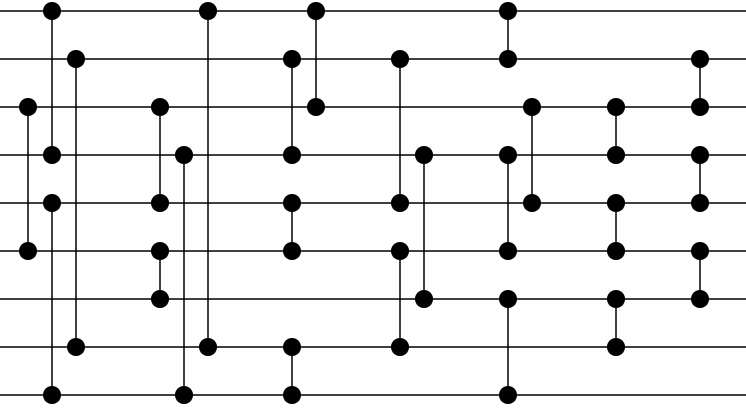
\includegraphics[scale=0.8]{images/Size8SortingNetwork}
\caption{Size 8 sorting network}
\label{fig:images/Size8SortingNetwork}
\end{figure}

\section{Generate and Prune}

\section{Generate and Prune Implementation}
\begin{algorithm}[H]
	\caption{Generate} 
	\begin{algorithmic}
	    \STATE $result \leftarrow \emptyset$
	    \STATE $N \leftarrow networks$
        \STATE $C \leftarrow comparators$
        \FOR{$n$ in $N$}
             \FOR{$c$ in $C$}
                \STATE $n' \leftarrow n\bigcup c$
                \IF {$n'$ is not redundant}
                    \STATE $result \leftarrow result \bigcup n'$
                \ENDIF
            \ENDFOR
            \STATE $n' \leftarrow $
        \ENDFOR
        \RETURN $result$
    \end{algorithmic}
\end{algorithm}

\begin{algorithm}[H]
	\caption{Prune} 
	\begin{algorithmic}
	    \STATE $R \leftarrow \emptyset$
	    \STATE $N \leftarrow networks$
        \FOR{$n$ in $N$}
             \FOR{$r$ in $R$}
                \IF {$r$ subsumes $n$}
                    \STATE $subsumed \leftarrow \TRUE$
                    \STATE break
                \ENDIF
                
                \IF {$n$ subsumes $r$}
                    \STATE $R \leftarrow R \setminus r$
                \ENDIF
            \ENDFOR
            \IF {$subsumed$ is \FALSE}
                \STATE $R \leftarrow R \bigcup n$
            \ENDIF
        \ENDFOR
        \RETURN $R$
    \end{algorithmic}
\end{algorithm}

\begin{algorithm}[H]
	\caption{Parallel Prune} 
	\begin{algorithmic}
	    \STATE $N \leftarrow networks$
	    \STATE $C \leftarrow Divide(N)$ \COMMENT{Divide N in as many Clusters as processor}
	    \STATE {Each processor performs:}
	    \STATE PRUNE($C_i$)
        \FOR{$c$ in $C$}
            \STATE Remove($c, C \setminus c$)
        \ENDFOR
        \RETURN $N$
    \end{algorithmic}
\end{algorithm}

\begin{algorithm}[H]
	\caption{Remove} 
	\begin{algorithmic}
	    \STATE $result \leftarrow \emptyset$
	    \STATE $N_i \leftarrow networks$
	    \STATE $N_j \leftarrow networks$
        \FOR{$n_i$ in $N_i$}
             \FOR{$n_j$ in $N_j$}
                \IF {$n_i$ subsumes $n_j$}
                    \STATE $N_j \leftarrow N_j \setminus n_j$
                \ENDIF
            \ENDFOR
        \ENDFOR
        \RETURN $N_j$
    \end{algorithmic}
\end{algorithm}

\section{Subsume Implementations}
\subsection{Permutations Enumeration}
\subsection{Bigraph Perfect Matchings}

\section{Heuristics}

\section{Conclusion}
\bibliography{references}
\end{document}
